\section{Testing}
%[[ include test plan and coverage data

For our testing we will be using JUnit. We will be focused on writing good tests rather than achieving a set percentage required to commit. We believe that this is a reliable way to ensure that good software is being developed. However, if we \textit{had} to give a numerical value, we decided that 80\% coverage would be sufficient to commit.

\begin{figure}[!hbt]
    \centering
    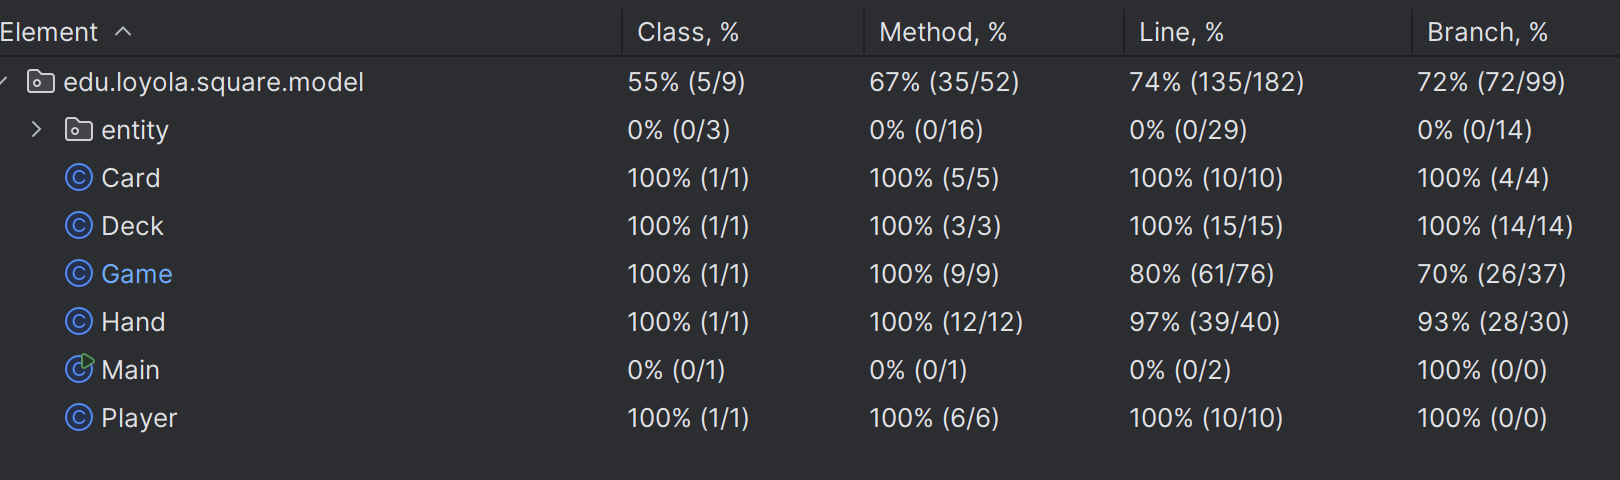
\includegraphics[width=1.0\linewidth]{figures/Coverage report (Model).png}
    \caption{Sprint 1 Coverage report (Note that the entity folder is being erroneously tested)}
    \label{Coverage report}
\end{figure}

%Briefly describe how you incorporated testing into each two week coding iteration. 
%What tool(s) proved useful? 
%What went well in terms of testing?
%What did not?

%]]
